\chapter{Results}

The result of this project is a functional prototype of an interactive fluid
simulator. A game designer can use the modified version of Blender to add
fluids into a game built with the Blender Game Engine. Basic functionality in
the simulation and game logic have been achieved, laying the groundwork for
more complex physical phenomenon as well as more interesting interactions.


\section{Performance}
    
The performance of the project was benchmarked on two modern GPUs, an NVIDIA
GTX 480 and an AMD FirePro V7800. The GTX 480 has 480 CUDA Cores and 1.5GB of
video memory while the FirePro V7800 has 1440 Stream processors and 2GB of
video memory. The number of cores and processors do not directly correspond to
performance, as can be seen from the timings presented in Figure 7.1.


In addition to benchmarking the project, the CUDA SPH implementation from
Krog\cite{Krog2010} was run on with the GTX 480. As shown in Figure 7.1 RTPS is
not yet as efficient as SimpleSPH. Comparisons with CPU implementations were
not carried out as the literature has shown the wide gap in performance makes
the CPU non-competitive.\cite{Hoetzlein}\cite{Krog2010}

Frames per Second (fps) is an important metric for most videogame players.  A
reasonable number for an interactive 3D game is 60fps, although 30fps is
sometimes deemed acceptable. Note that movies play at 24fps. The performance of
the simulations are compared with frames per second, while analysis of the
routines within the simulation is measured in milliseconds. Updating one frame
takes 17ms to obtain a framerate of 60fps, and 33ms at 30fps. In the following
timings, when using fps a higher number is desirable while when measuring in
milliseconds a lower number is preferred.

\pagebreak

\begin{figure}[!htc]
 		\centering
        \subfloat[maximum number of particles equal to number of particles]{\label{fig:fps_num}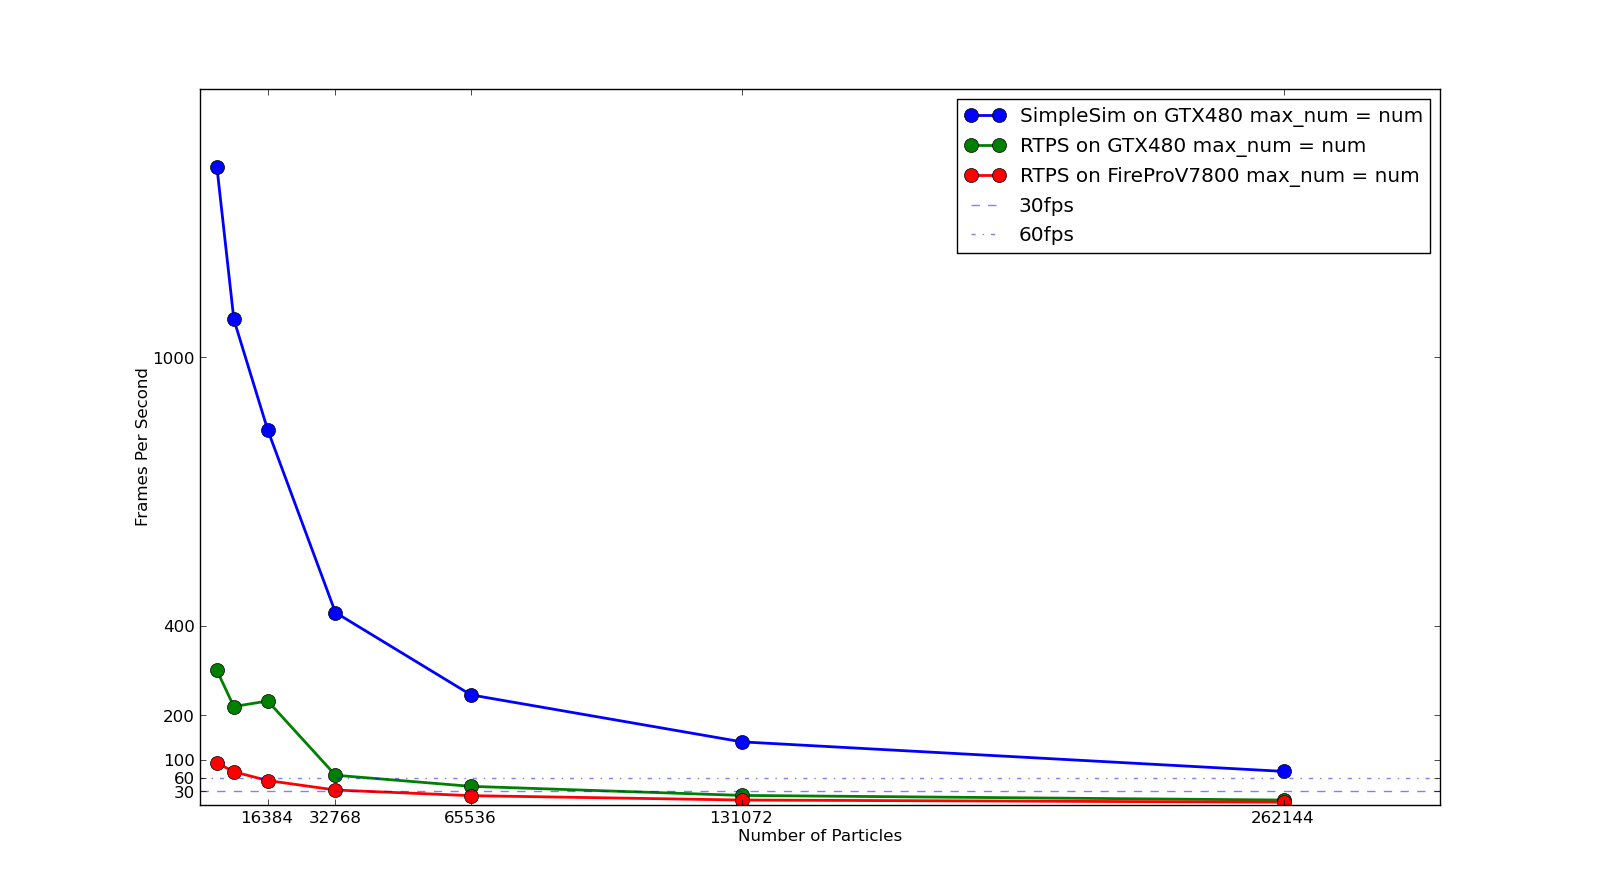
\includegraphics[scale=0.5]{figures/maxnum_eq_num_fps.png}}
        \\
        \subfloat[maximum number of particles equal to 1 million]{\label{fig:fps_1mill}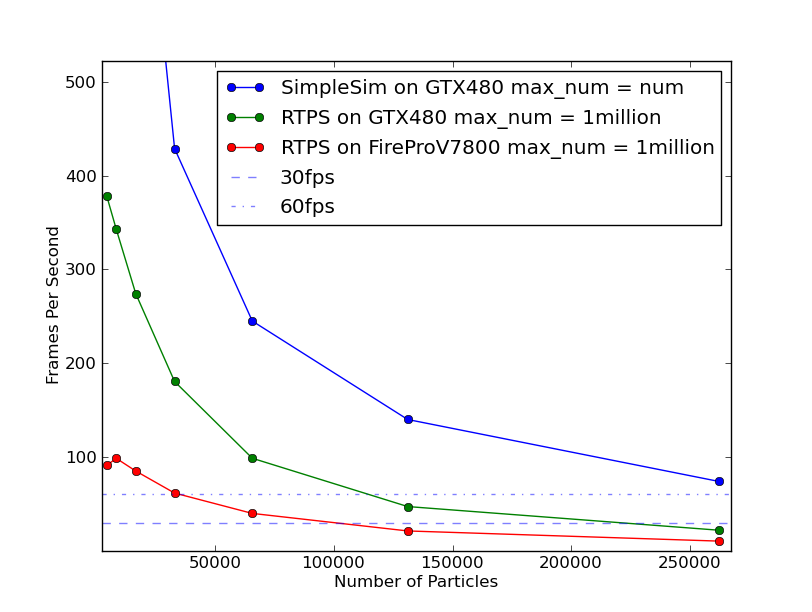
\includegraphics[scale=0.5]{figures/maxnum_eq_1mill_fps.png}}
        \caption{Frame Rates}
        \label{fig:fps}
\end{figure}

\pagebreak

For the timings in \ref{fig:fps_num} the only parameter varied is the maximum number of particles.
For each case the maximum number of particles is emitted and the timing of each
function call is averaged over 1000 iterations.

One logical use scenario would involve setting a large maximum number of
particles and only using a relatively small subset of them. This will make the
radius of each particle smaller if the domain size remains fixed, allowing the
user to get a more detailed simulation. It turns out that this use case is much
more efficient than setting the maximum number of particles to the amount to be
used as can be seen in Figure \ref{fig:fps_1mill}.

One can see from Figure \ref{fig:kernel_time} that the Density and Force calculations are by far
the most expensive routines. These routines have the most memory accesses, and
the more neighbors that each particle must calculate the more memory accesses
these routines use. It is important to note that the Sorting routine
contributes a non-trivial amount of time to the computation.

%\pagebreak

\begin{figure}[!htc]
 		\centering
		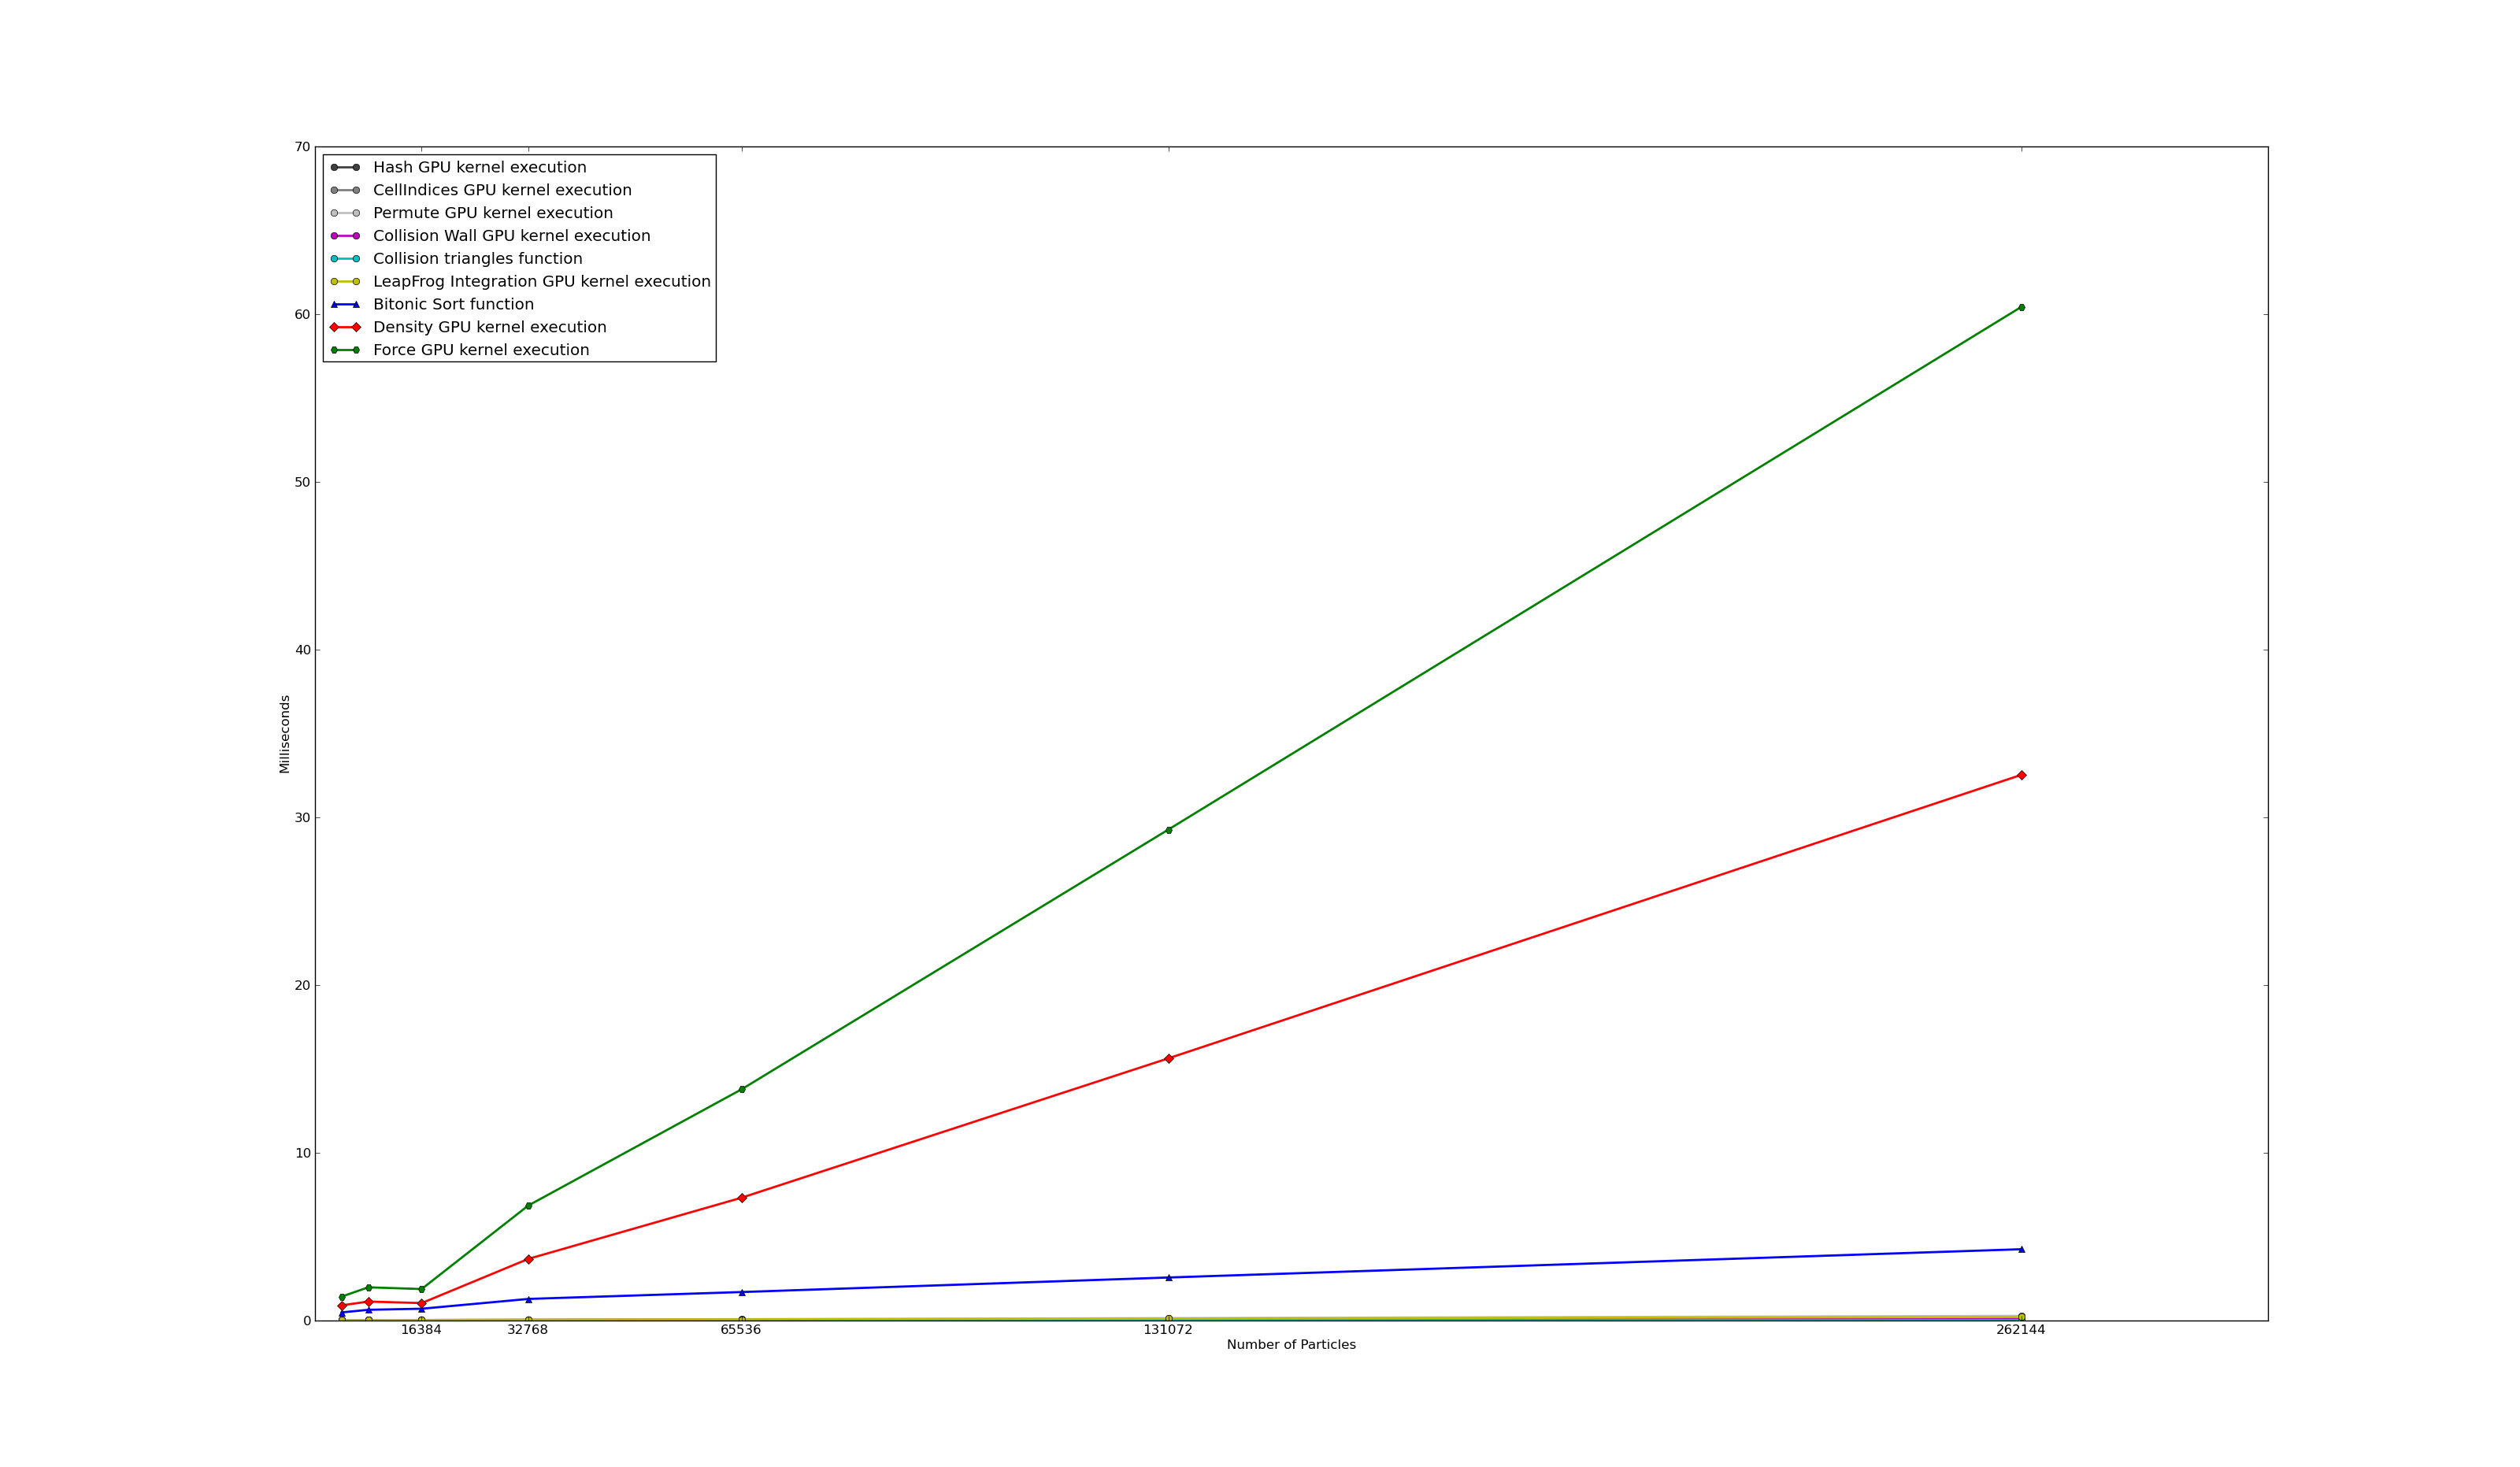
\includegraphics[scale=0.35]{figures/nv_kernel_num.png}
        \caption{ GPU timings for each kernel }
        \label{fig:kernel_time}
\end{figure}

Figure \ref{fig:kernel_time} shows a linear increase in cost as the number of
particles increase past 16384. Below this number increasing the particles has a
negligable effect on the cost. This is most likely due to the overhead of
launching the kernels overshadowing the small amount of memory accesses and
computations required by such a small amount of particles. 

\pagebreak

Figure \ref{fig:pies} shows the proportion of time taken by the most expensive
kernels on each video card using 262144 particles. The proportions are similar
for each card, with the sort contributing more on the AMD hardware.

\begin{figure}[!htc]
 		\centering
        \subfloat[NVIDIA]{\label{fig:nv_pie}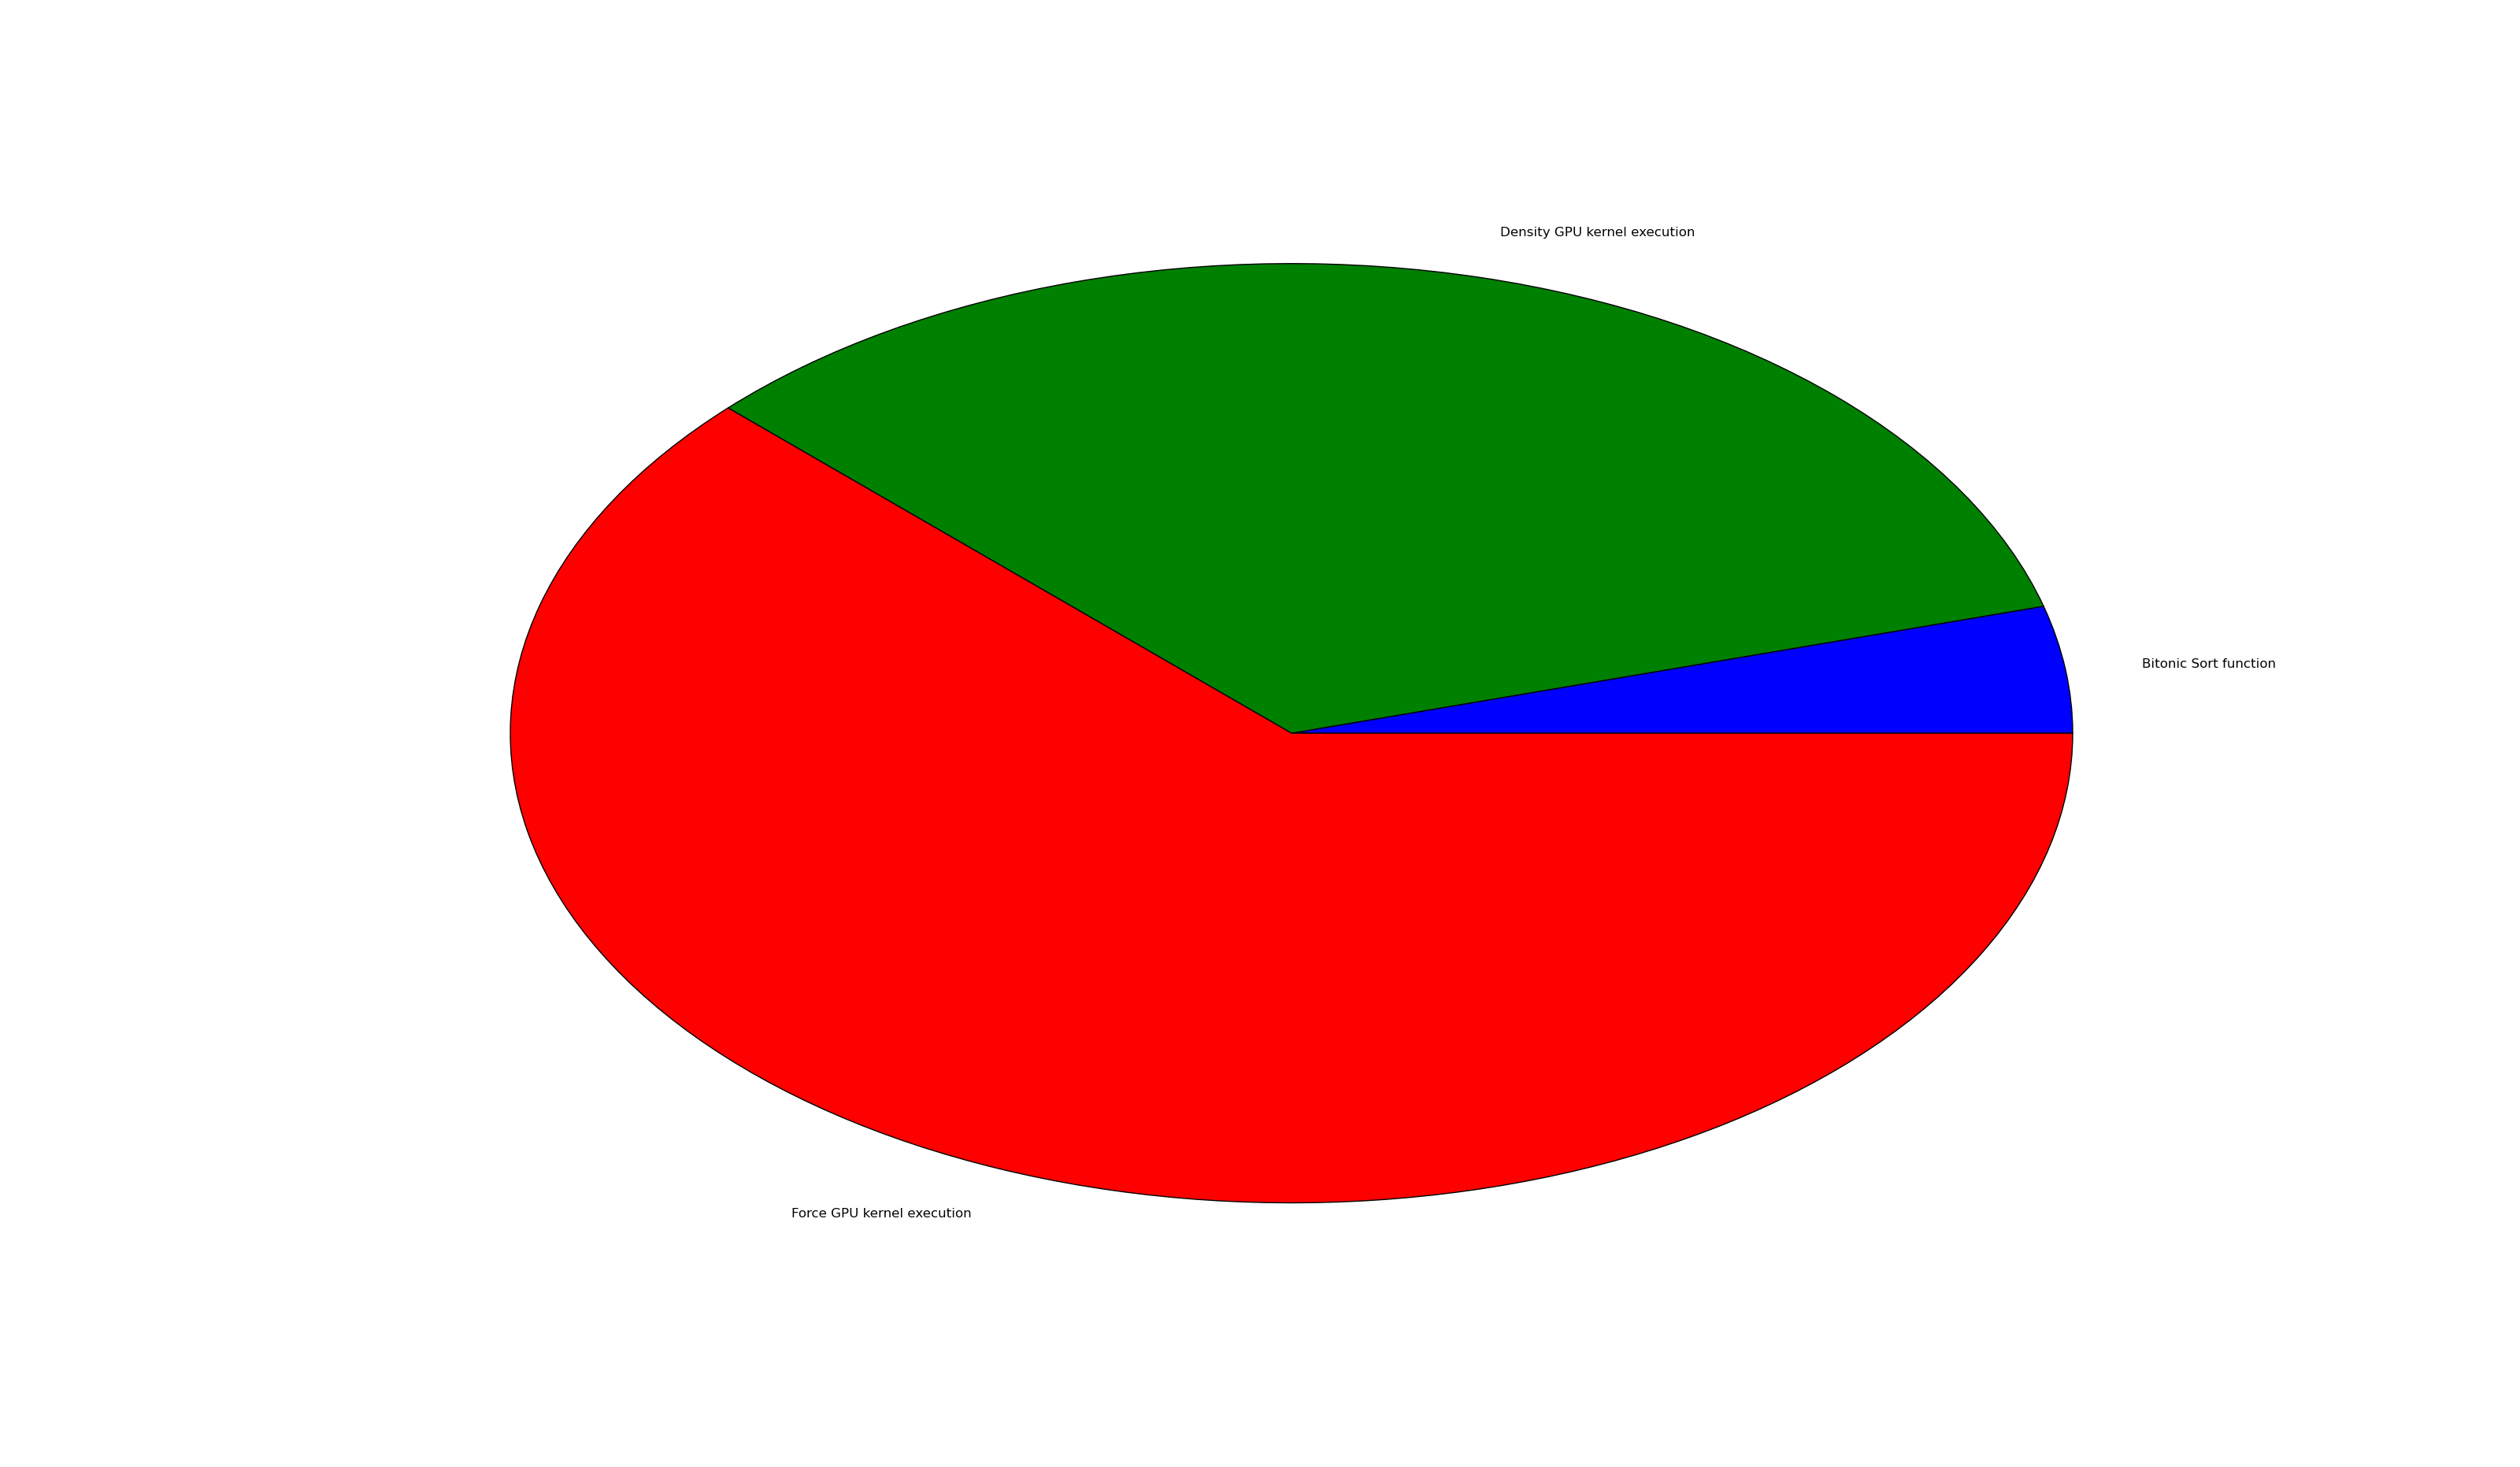
\includegraphics[scale=0.2]{figures/nv_pie.png}}
        \subfloat[AMD]{\label{fig:ati_pie}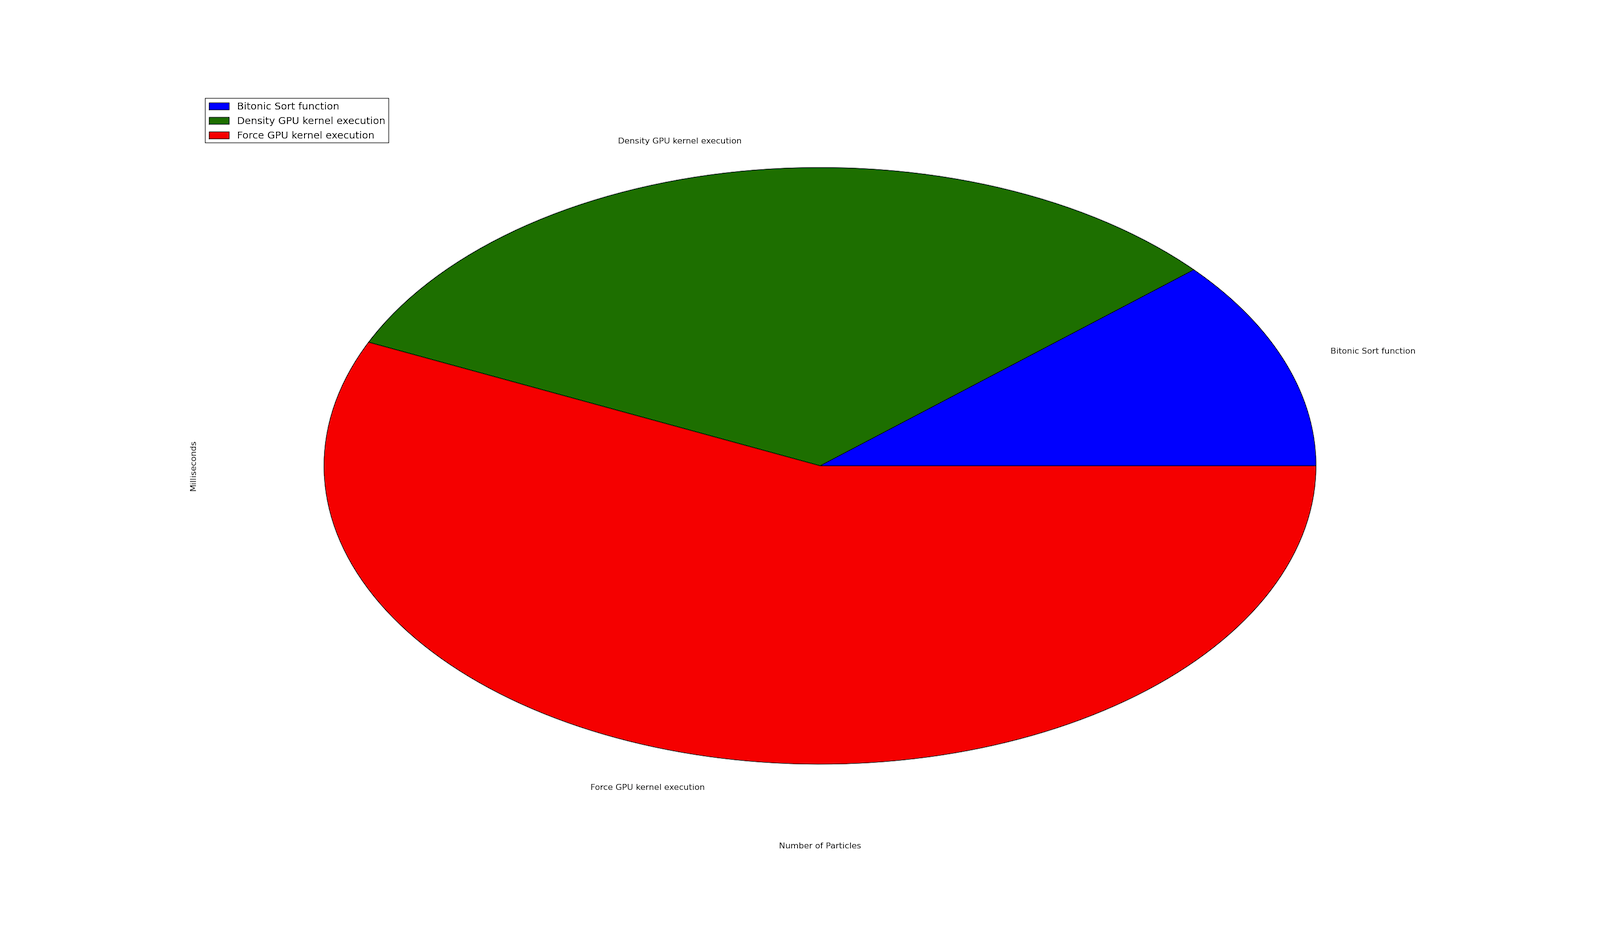
\includegraphics[scale=0.2]{figures/ati_pie.png}}
        \caption{ Proportion of GPU timings for the most expensive kernels on each card }
        \label{fig:pies}
\end{figure}

\section{Data Structures}
The data structures used on the GPU are given as follows:

\begin{cppcode}{0}
        //Depend on number of particles
        Buffer<float4>      cl_position_u;
        Buffer<float4>      cl_position_s;
        Buffer<float4>      cl_color_u;
        Buffer<float4>      cl_color_s;
        Buffer<float4>      cl_velocity_u;
        Buffer<float4>      cl_velocity_s;
        Buffer<float4>      cl_veleval_u;
        Buffer<float4>      cl_veleval_s;
        Buffer<float>       cl_density_s;
        Buffer<float4>      cl_force_s;
        Buffer<float4>      cl_xsph_s;
        Buffer<unsigned int>         cl_sort_hashes;
        Buffer<unsigned int>         cl_sort_indices;
        Buffer<unsigned int>         cl_sort_output_hashes;
        Buffer<unsigned int>         cl_sort_output_indices;

        //Depend on number of grid cells
        Buffer<unsigned int>         cl_cell_indices_start;
        Buffer<unsigned int>         cl_cell_indices_end;
\end{cppcode}

Using the standard size of single precision floats and unsigned ints of 4
bytes, each particle requires $45*4$ or $180$ bytes of memory. Each grid cell
requires $8$ bytes of memory. With this configuration a simulation with 65,536
particles will require a grid with 12,167 cells for a total of 11.34MB. A
simulation with 1,048,576 particles will require a grid with 132,651 cells and a
total of 181MB. These numbers do not come close to saturating the 2GB of memory
available on modern GPUs.


\section{Community}
An important aspect of this project is adoption by the game design community.
Acceptance by the Blender community entails benefits such as user generated
tutorials and developer support. The project has enjoyed a preliminary amount
of success in this regard, being featured on the primary news source for
the Blender community.\footnote{
\url{http://www.blendernation.com/2011/01/03/fluids-in-real-time-with-opencl/}
\\ 
\url{
http://www.blendernation.com/2011/04/20/ian-johnson-fluid-simulation-blender-game-engine-using-opencl/
} }

Builds were compiled for the Windows, Mac and Linux operating systems and
distributed to members of the community for testing. These members have already
provided valuable feedback, crash reports and even demos.\footnote{ \url{http://www.youtube.com/watch?v=s2QBRazykEA}} 

\begin{figure}[!htc]
 		\centering
		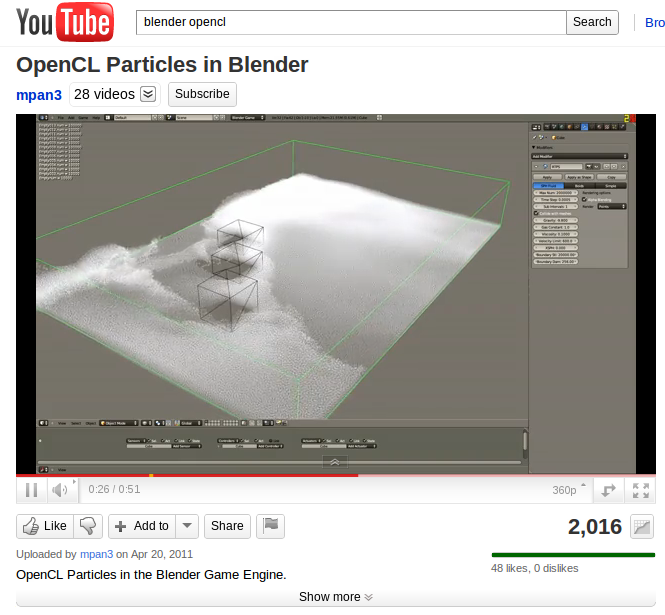
\includegraphics[scale=0.5]{figures/youtube.png}
        \caption{ Artist demo }
		\label{fig:mpan}
\end{figure}

The project has also recieved support from developers with regards to
integrating the RTPS library with Blender. As the code improves and the
integration becomes tighter it is expected that more developers will be willing
and able to help.


\section{Screen Shots}

Selected screen shots of the Blender Game Engine with the RTPS library in action.

\begin{figure}[!htc]
 		%\centering
		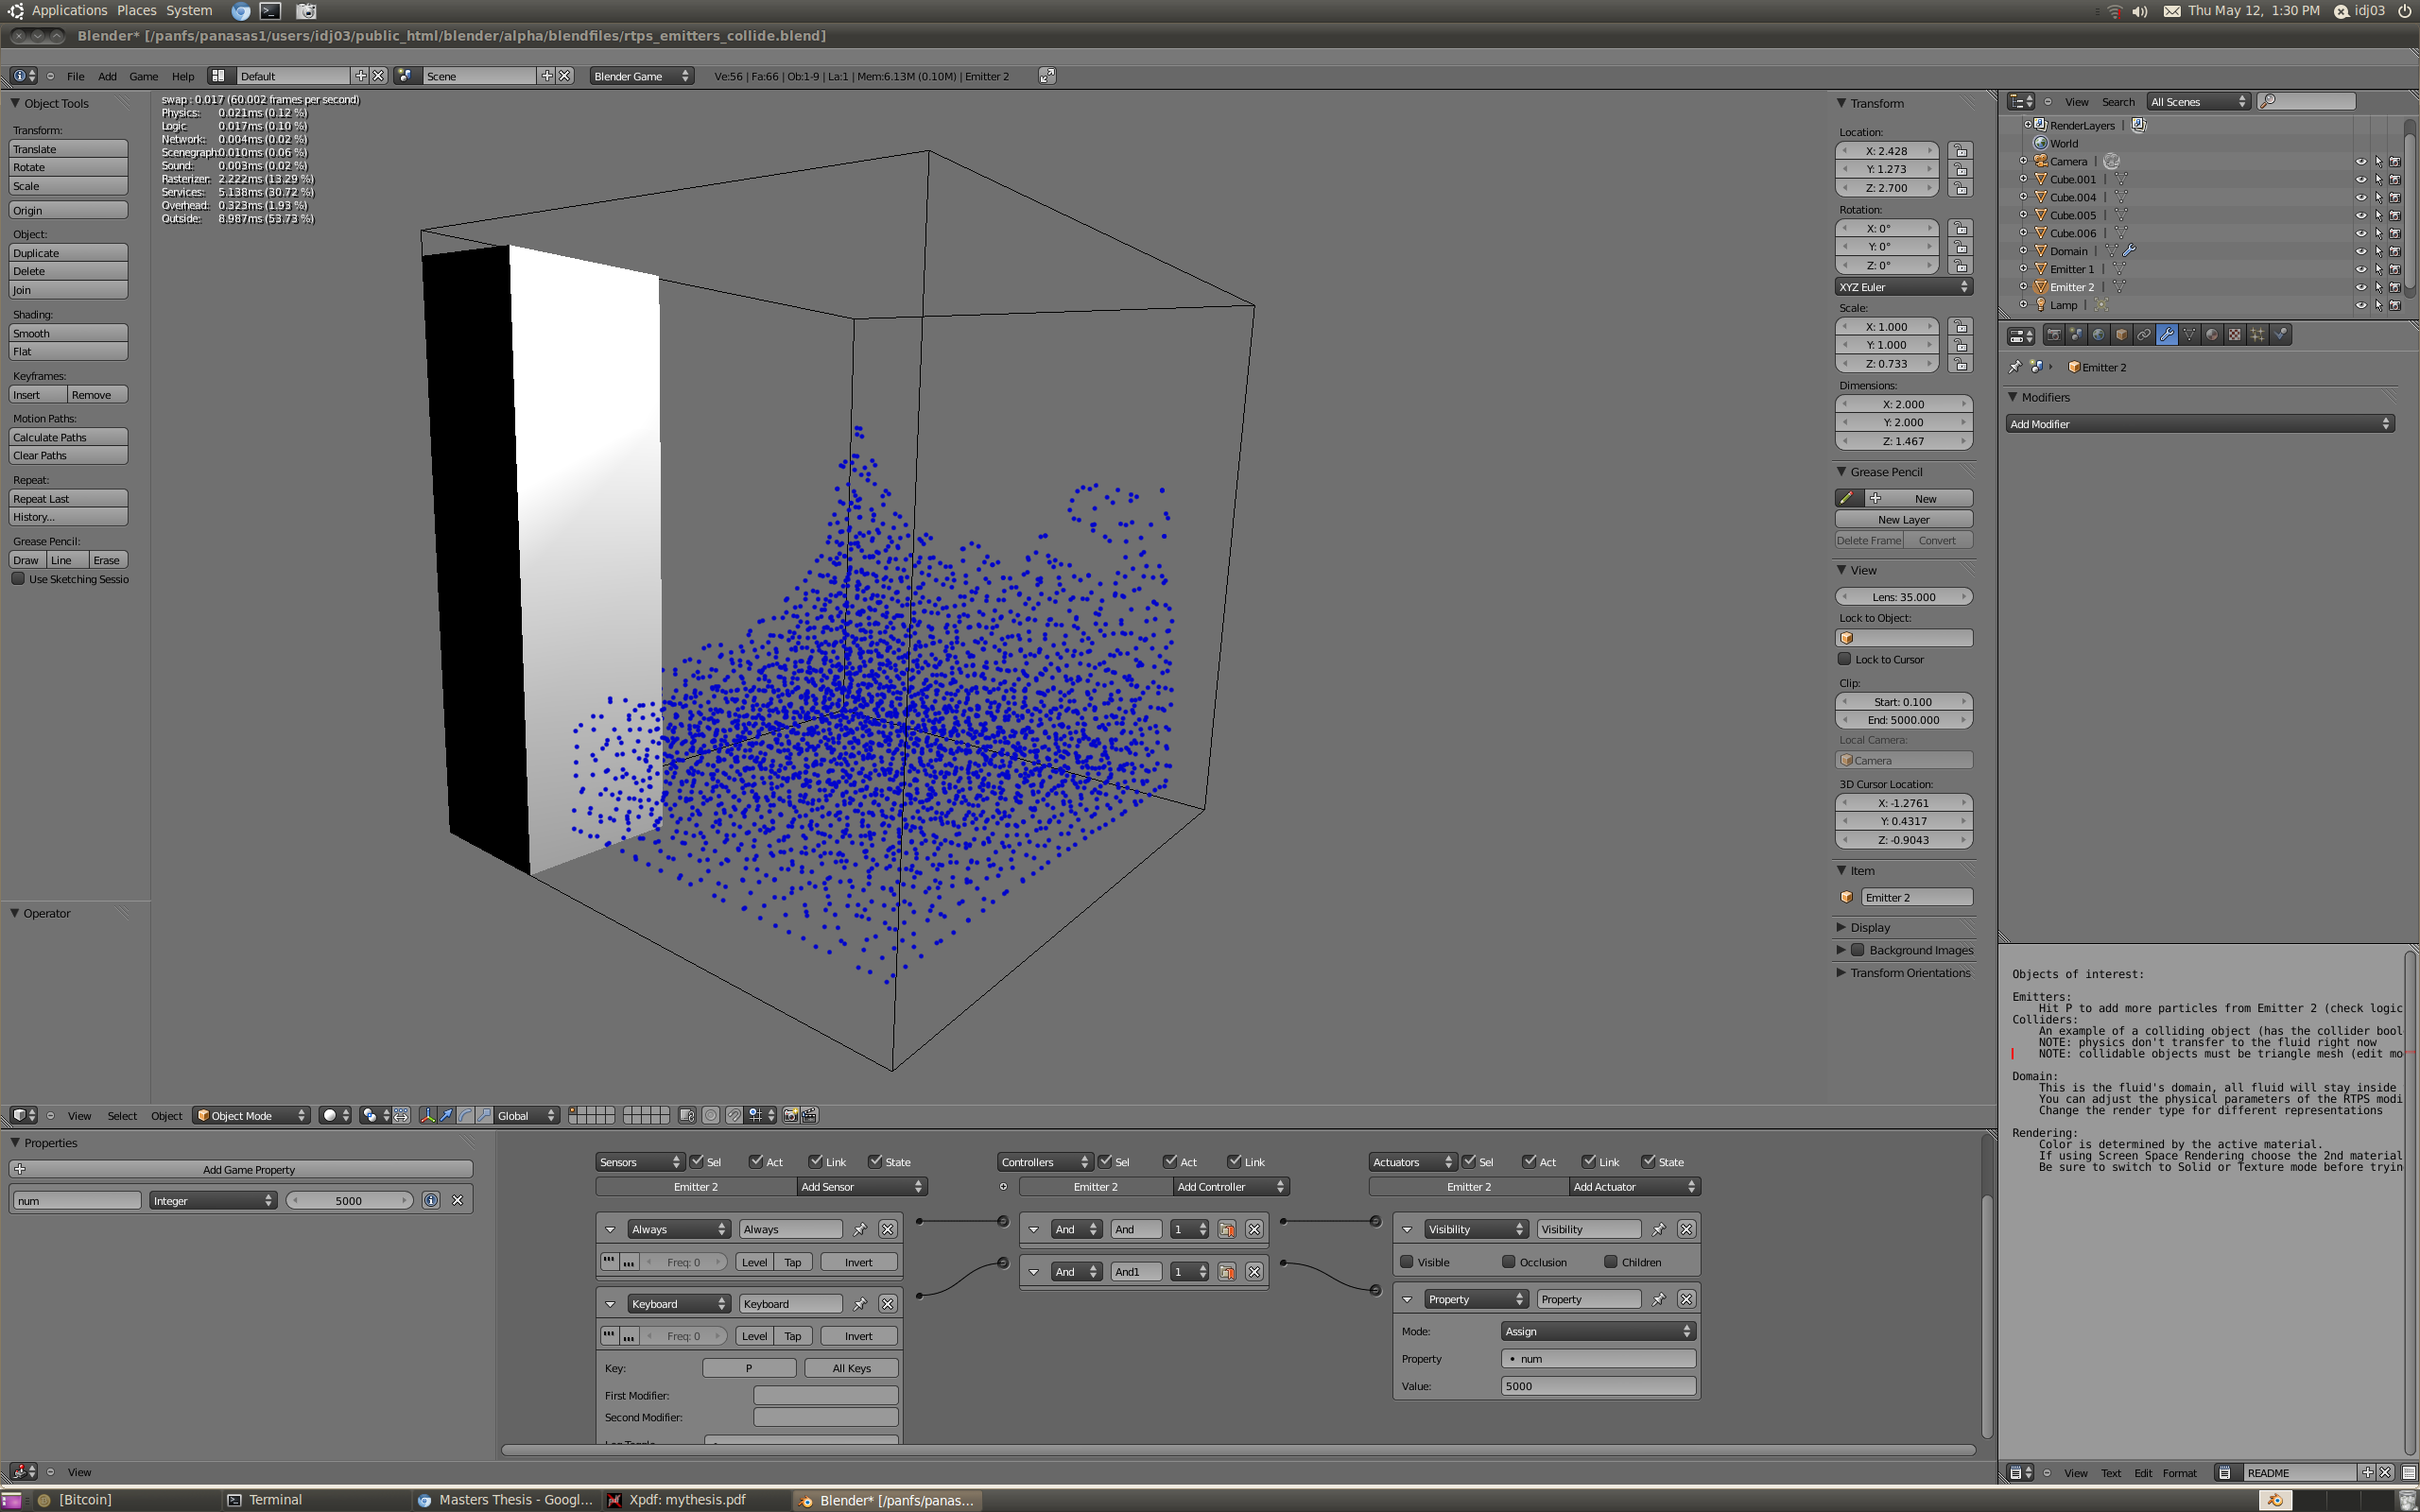
\includegraphics[scale=0.17]{figures/dam_break.png}
        \caption{ Dam break with 65k particles maximum }
		\label{fig:dam_break}
\end{figure}

\pagebreak

\begin{figure}[!htc]
 		%\centering
		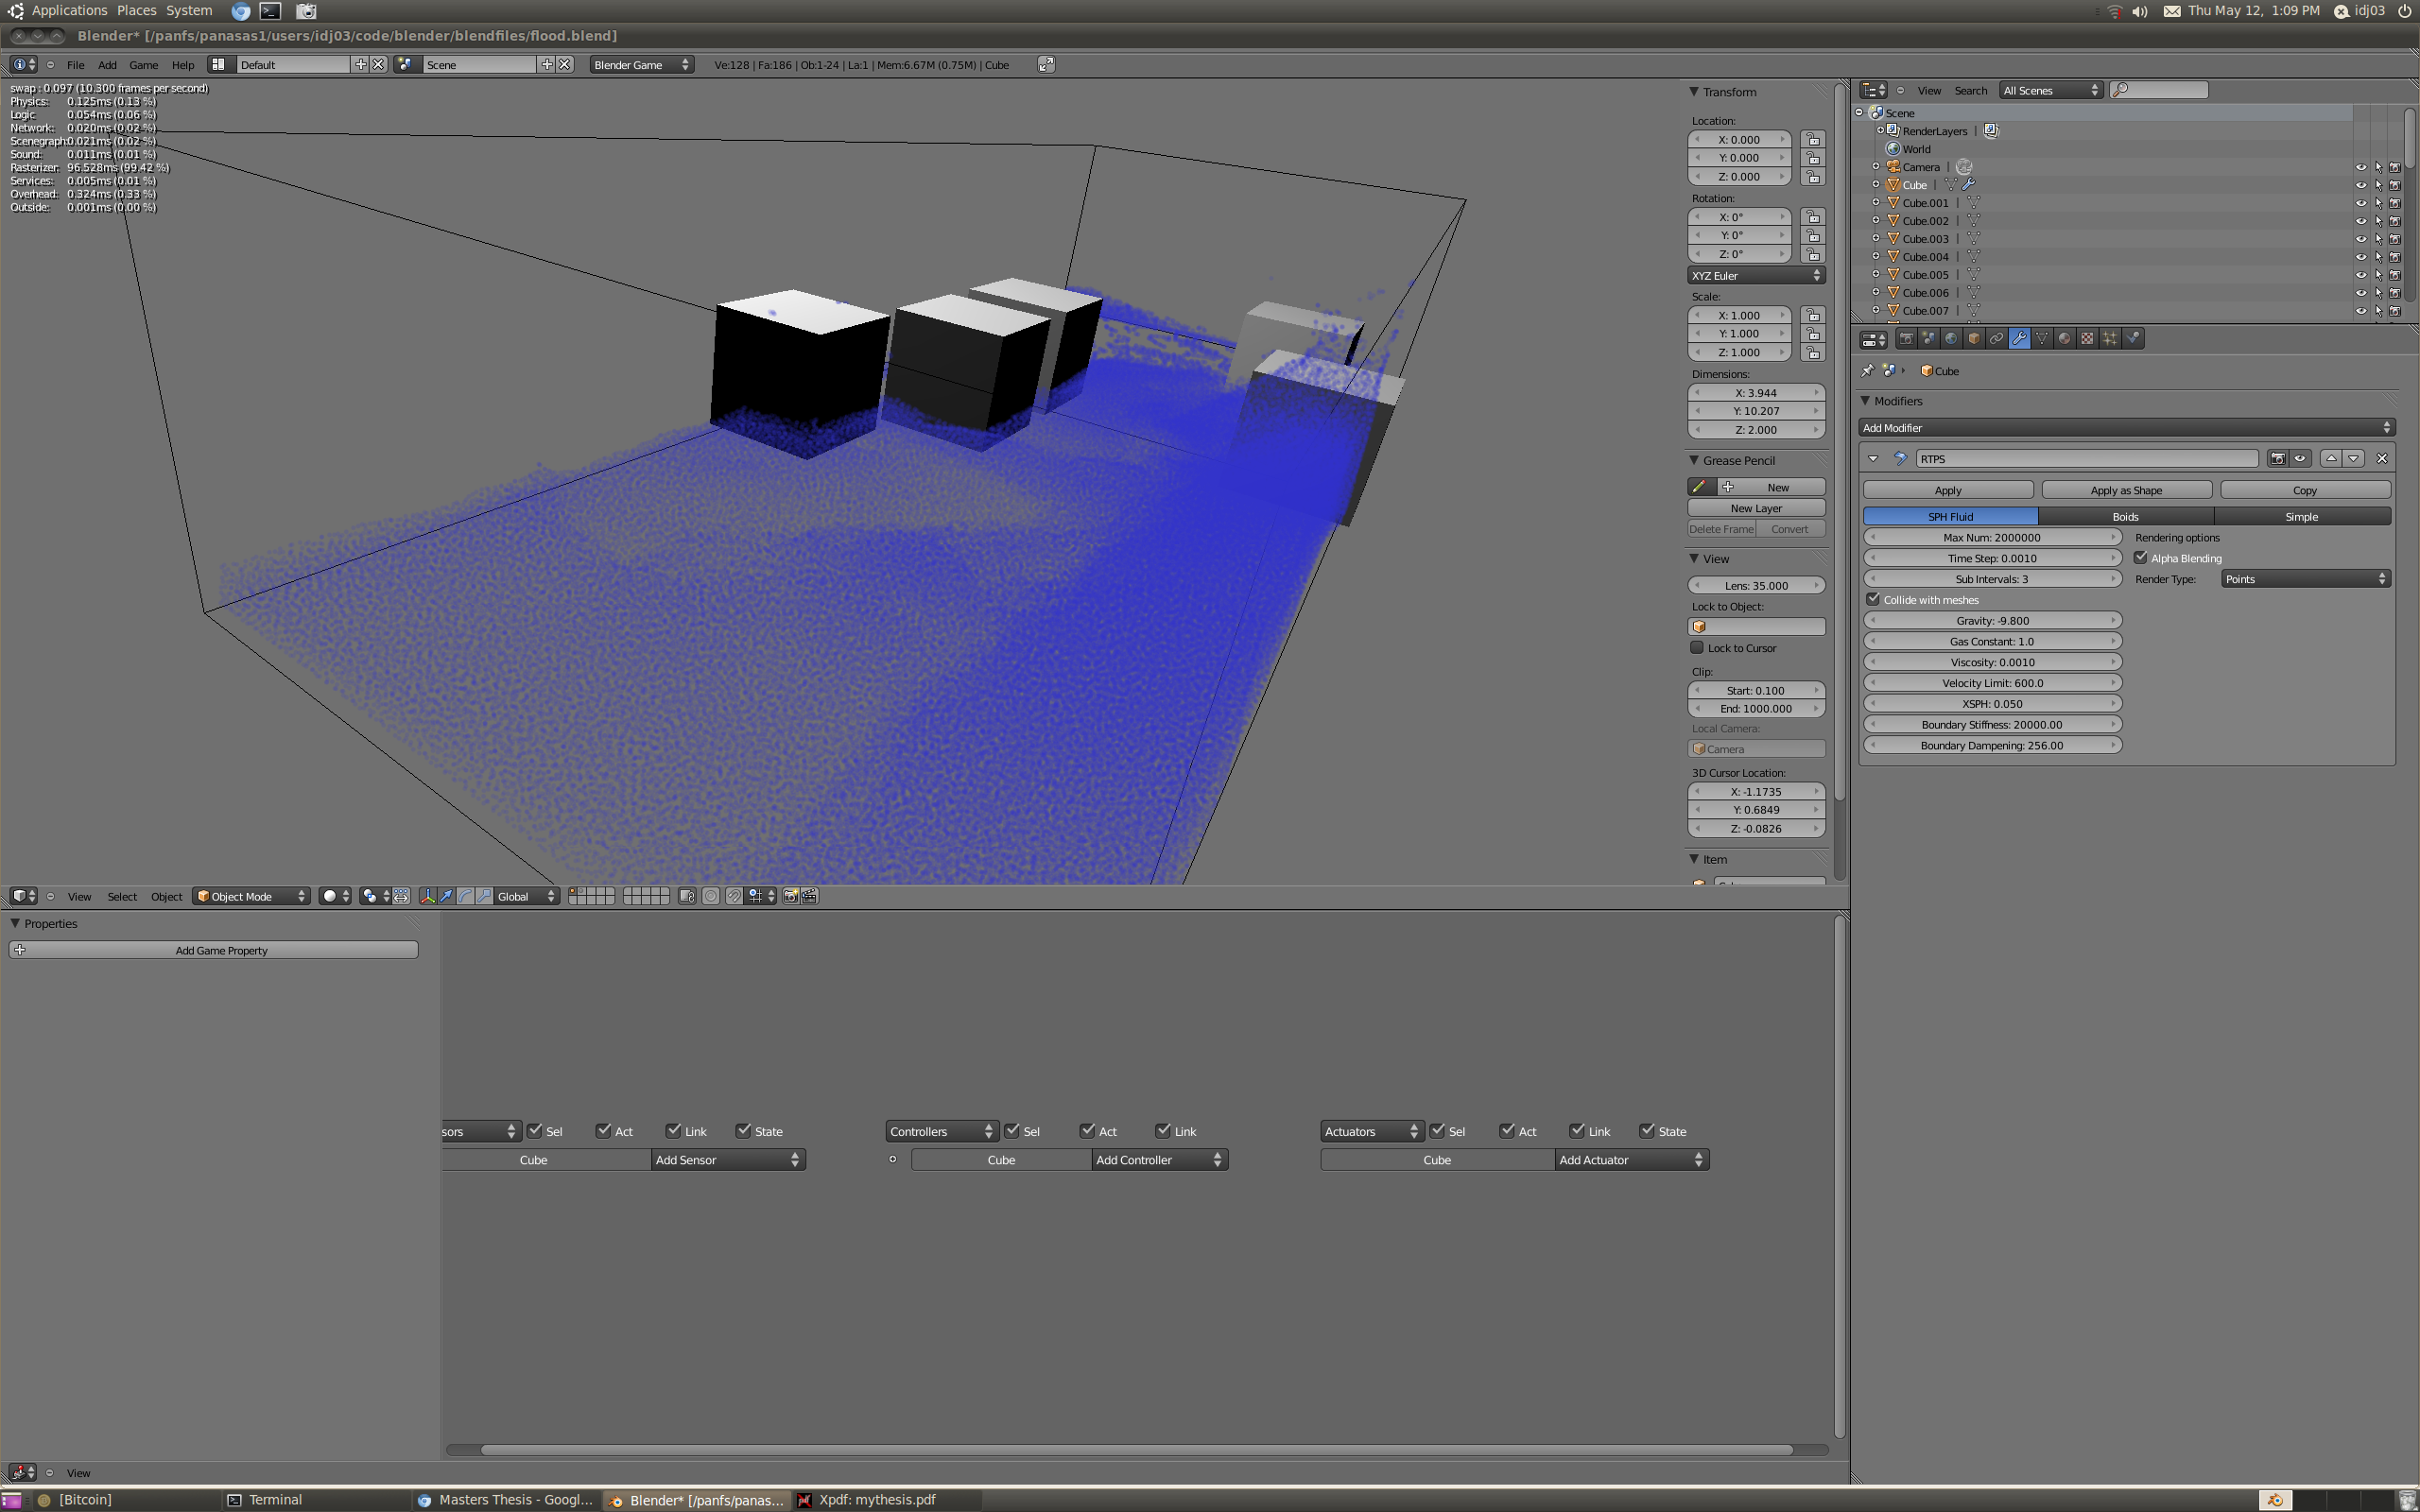
\includegraphics[scale=0.17]{figures/flood1.png}
        \caption{ 100k particles colliding with boxes. }
		\label{fig:flood1}
\end{figure}

\pagebreak
\begin{figure}[!htc]
 		%\centering
		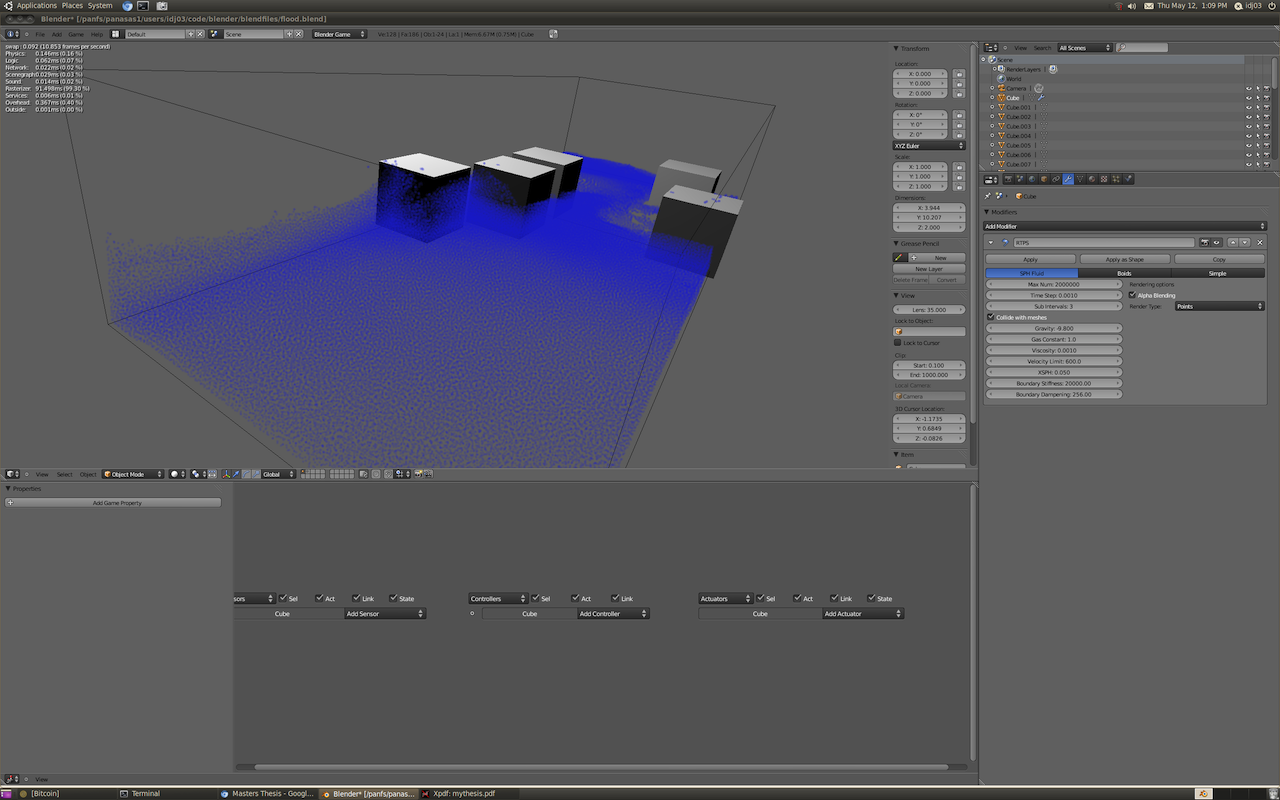
\includegraphics[scale=0.17]{figures/flood2.png}
        \caption{ 100k particles colliding with boxes. }
		\label{fig:flood2}
\end{figure}

\pagebreak
\clearpage

\subsection{Videos}

Videos have been recorded throughout the process of this research and are
available on the web. These videos are listed in reverse chronological order
from most recent to oldest. \\
\url{http://vimeo.com/21743717} \\
\url{http://vimeo.com/19794084} \\
\url{http://vimeo.com/17906099} \\
\url{http://www.youtube.com/watch?v=YvQFgY4kY68} \\
\url{http://www.youtube.com/watch?v=kXi70eaClnQ} \\
\url{http://www.youtube.com/watch?v=lP6zfAVm7B0} \\



